\documentclass[10pt]{article}
\usepackage{NotesTeX} %/Path/to/package should be replaced with package location
\usepackage{lipsum}
\usepackage{tensor}
\usepackage{amsmath,amsthm,amssymb}
\usepackage{hyperref}
\usepackage{physics}
\input{undertilde}

\newcommand{\bs}{\textbackslash}


\title{{\Huge General Relativity}\\{\Large{Class 25 - March 27, 2020}}} %replace with class number
\author{Mohammad Shobaki}

\emailAdd{Mohammadshobaki@utexas.edu} %replace with your email
\begin{document}
    \maketitle
    \flushbottom
    \newpage
    \pagestyle{fancynotes}
    %\part{HELLO \LaTeX\,}
	%Use the uncompiled version of this document in itself as a \LaTeX\, style guide for the class you'll be responsible for.

     \paragraph{}In general, equations of the form ${G}_{\mu\nu}=8\pi{T}_{\mu\nu}$ cannot be solved exactly. In practice, with a given ${T}_{\mu\nu}$, we usually use an approximation or settle to solve a simpler case. This tends to involve assumed symmetries for the spacetime. With enough assumptions, we can utilize known techniques to solve the problem. The subject of this lecture is an extreme case known as maximally symmetric spacetimes. These are spacetimes with the highest number of symmetries possible. These spacetimes look the same at every point, and look the same in every direction, i.e. homogeneous and isotropic. 
     
     \section{Maximally Symmetric Spacetimes}
     \paragraph{}The simplest example of a maximally symmetric spacetime is Minkowski space. In Minkowski space, we have a number of transformations that preserve the metric ${\eta}_{\mu\nu}$. There are 4 translations: ${x}^{\mu} \rightarrow {x}^{\mu} + {a}^{\mu}$, and there are 6 Lorentz transformations (3 rotations and 3 boosts): ${x}_{\mu} \rightarrow {{\Lambda}^{\mu'}}_{\nu} {x}^{\nu}$. There are 10 symmetries here in total. This is the maximum possible for a four dimensional spacetime, so Minkowski space is a maximally symmetric spacetime.
     
     \paragraph{} The maximum number of symmetries in an n-dimensional space can have can be thought of as follows. There are n dimensions, so there are n possible translations. There are $n$ axes that can be rotated into $n-1$ other axes, so there are $n(n-1)$ rotations, but a rotation from x into y is simply the opposite of a rotation from y into x, so we have to divide by two, $\frac{n(n-1)}{2}$. This leads to a total of $n + \frac{n(n-1)}{2} = \frac{n(n+1)}{2}$ possible symmetries. For $n=4$, we have $10$ symmetries which agrees with what we knew about Minkowski space. Each symmetry corresponds to a Killing vector field in the spacetime. 
     
     \paragraph{}Applying the above formula, we see that in a 2-dimensional space, there are 3 symmetries. As an example, in ${R}^{2}$, there are 2 translations and 1 rotation. In a 3-dimensional space, there are 6 symmetries, which agrees with our understanding of ${R}^{3}$ in which there are 3 translations and 3 rotations. A less trivial case is that of ${S}^{2}$, the surface of a sphere, where ${ds}^{2} = {d\theta}^{2} + {sin}^{2}(\theta){d\phi}^{2}$. Here, there are 3 killing vectors, which are the three rotations in figure 1, so ${S}^{2}$ is maximally symmetric.
     
      \begin{figure}[h]
         \centering
         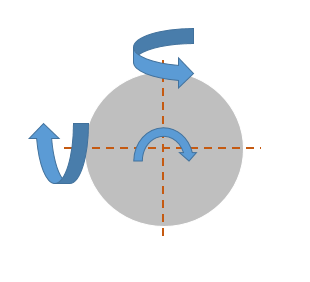
\includegraphics[width = .3\textwidth]{sphere_rotations.png}
         \caption{Rotatiosn for ${S}^{2}$}
         \label{fig:my_label}
     \end{figure}
     
     In a Euclidean signature space ${S}^{n}$(all + in the metric), the n-dimensional sphere is maximally symmetric.  
     
     \section{Curvature of Maximally Symmetric Space(time)s}
     \paragraph{}Moving into some local Lorentz frame at some point p in a maximally symmetric spacetime, the curvature tensor must look the same in every direction. The metric ${g}_{\mu\nu}$ in this frame remains invariant under Lorentz transformations.
     
      \begin{figure}[h]
         \centering
         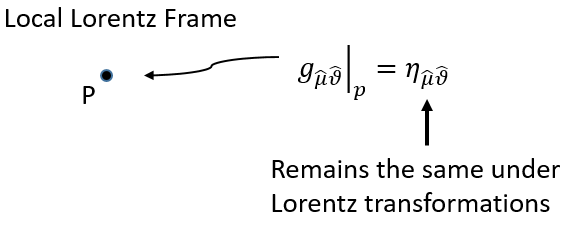
\includegraphics[width = .6\textwidth]{remains_same_at_point.png}
         \label{fig:my_label}
     \end{figure}
     
     We would want this property to also be true for the curvature tensor ${R}_{\hat{\mu}\hat{\nu}\hat{\rho}\hat{\sigma}}$. The curvature should look the same no matter how the space is rotated or boosted at this point. This means the curvature should be built out of Lorentz invariant objects. The only objects we know of that behave this way are ${\eta}_{\hat{\mu}\hat{\nu}}$, ${\epsilon}_{\hat{\mu}\hat{\nu}\hat{\rho}\hat{\sigma}}$, and ${{\delta}^{\hat{\mu}}}_{\hat{\nu}}$. It turns out that the natural choice is to build ${R}_{\hat{\mu}\hat{\nu}\hat{\rho}\hat{\sigma}}$ out of combinations of the metric. 
     
     \paragraph{} ${R}_{\hat{\mu}\hat{\nu}\hat{\rho}\hat{\sigma}}$ will be built out of ${\eta}_{\hat{\mu}\hat{\nu}}$ in such a way as to respect the properties of the Riemann tensor. There are four lower indices in ${R}_{\hat{\mu}\hat{\nu}\hat{\rho}\hat{\sigma}}$, so two copies of the metric will be used. The curvature is symmetric in interchange of $(\hat{\mu}\hat{\nu})$ and $(\hat{\rho}\hat{\sigma})$ and antisymmetric in interchange of $\hat{\mu}$ and $\hat{\nu}$ or $\hat{\rho}$ and $\hat{\sigma}$. The following suffices to achieve these properties.
     
     \begin{equation}
         {R}_{\hat{\mu}\hat{\nu}\hat{\rho}\hat{\sigma}} \propto  {\eta}_{\hat{\mu}\hat{\rho}}{\eta}_{\hat{\nu}\hat{\sigma}} - {\eta}_{\hat{\nu}\hat{\rho}}{\eta}_{\hat{\mu}\hat{\sigma}}
     \end{equation}
     
     If this formula can be written in one coordinate system, it must be so in all coordinate systems, so at this point, the following is true.  
     \begin{equation}
         {R}_{\hat{\mu}\hat{\nu}\hat{\rho}\hat{\sigma}} \propto  {g}_{\hat{\mu}\hat{\rho}}{g}_{\hat{\nu}\hat{\sigma}} - {g}_{\hat{\nu}\hat{\rho}}{g}_{\hat{\mu}\hat{\sigma}}
     \end{equation}
     Furthermore, since a maximally symmetric spacetime is the same everywhere, this relationship must hold everywhere. 
      \begin{equation}
         {R}_{\mu\nu\rho\sigma} = \kappa({g}_{\mu\rho}{g}_{\nu\sigma} - {g}_{\nu\rho}{g}_{\mu\sigma})
     \end{equation}
     Where $\kappa$ is some constant.
     
     \paragraph{} The Ricci tensor, ${R}_{\mu\nu}$, and the Ricci scalar, $R$, can be computed in terms of $\kappa$.
     
         \begin{equation}
         {R}_{\nu\sigma} = {{R}^{\alpha}}_{\nu\alpha\sigma} &= {g}^{\alpha\beta}\kappa({g}_{\alpha\beta}{g}_{\nu\sigma} - {g}_{\nu\beta}{g}_{\alpha\sigma})
         &= \kappa(n{g}_{\nu\sigma} - {{g}_{\nu}}^{\alpha}{g}_{\alpha\sigma}) = \kappa(n-1){g}_{\nu\sigma}
     \end{equation}
     
     so, 
     \begin{equation}
         {R}_{\mu\nu} = \kappa(n-1){g}_{\mu\nu}
     \end{equation}
     
     For the Ricci scalar,
    \begin{equation}
             R = {g}^{\mu\nu}{R}_{\mu\nu} = \kappa(n-1) {{g}^{\mu}}_{\mu} = \kappa n(n-1)
    \end{equation} 

     so
    \begin{equation}
        \kappa = \frac{R}{n(n-1)}
    \end{equation}
    
    Putting the above result together, 
    
    \begin{equation}
        {R}_{\mu\nu\rho\sigma} = \frac{R}{n(n-1)}({g}_{\mu\rho}{g}_{\nu\sigma} - {g}_{\nu\rho}{g}_{\mu\sigma})
    \end{equation}
    
    and 
    \begin{equation}
        {R}_{\mu\nu} = \frac{R}{n-1}{g}_{\mu\nu}
    \end{equation}
    
    These are the Riemann and Ricci tensors for any maximally symmetric space. We have determined this so far without ever specifying the form of ${g}_{\mu\nu}$. Usually when solving Einstein's equation, we need to specify a set of coordinates from the beginning to make progress; however, we have determined the form of the spacetime's curvature in a completely coordinate independent manner. 
    
    \paragraph{}We will see soon that everything here depends on R. The case of $R=0$, ${R}_{\mu\nu\rho\sigma} = 0$, corresponds to flat space. There are two other cases: $R > 0$ and $R < 0$. For \underline{spaces}, constant $R>0$ corresponds to n-dimensional spheres, ${S}^{n}$. Constant $R<0$ corresponds to n-dimensional hyperboloids, ${H}^{n}$. ${H}^{2}$ cannot be embedded in 3-dimensional flat space in contrast to ${S}^{2}$, but a sense of it can be achieved with a saddle shape since it is negatively curved in every direction. 
     
    \begin{figure}[h]
         \centering
         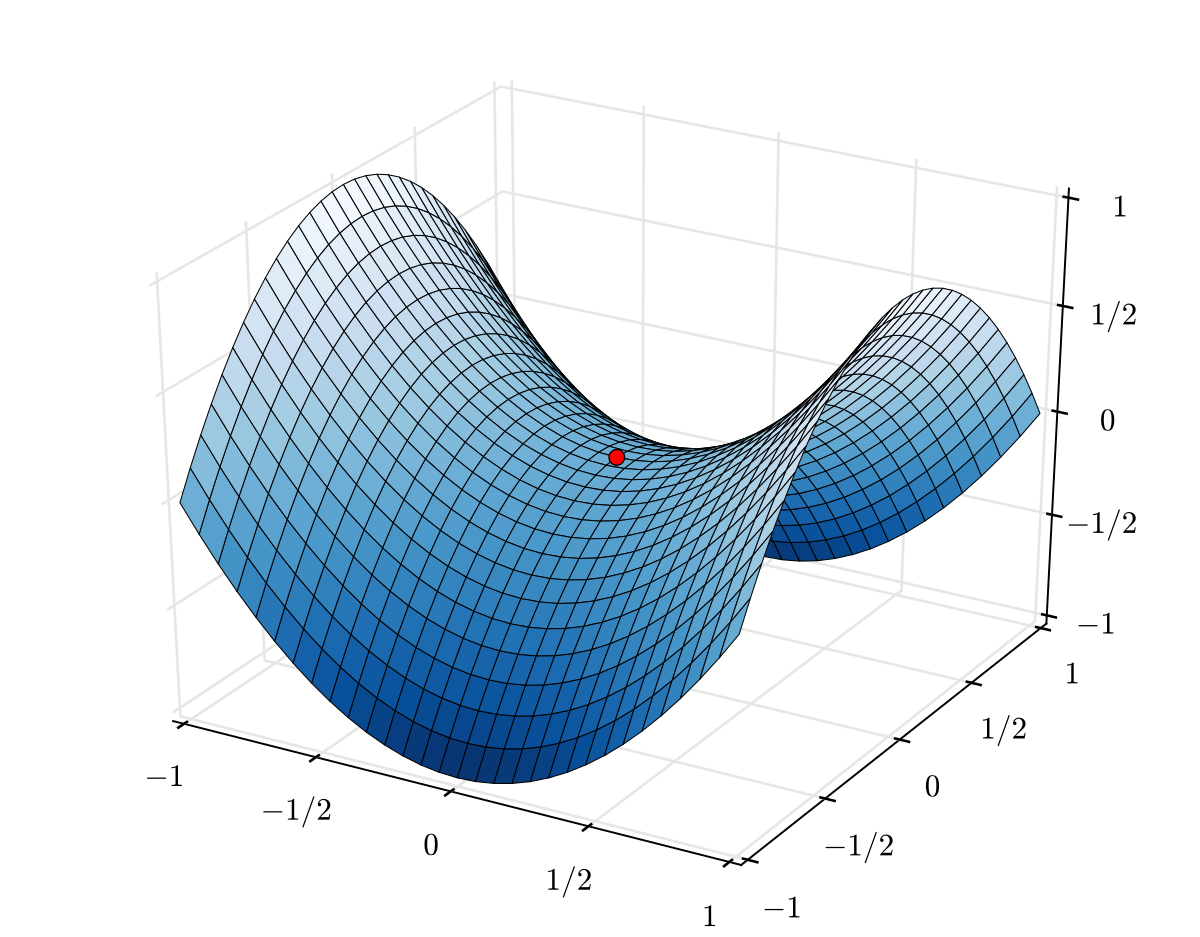
\includegraphics[width = .5\textwidth]{Saddle_point.svg.png}
        \caption{Visual aid for imagining ${H}^{2}$}
         \label{fig:my_label}
    \end{figure}
    
    In a \underline{spacetime}, constant $R>0$ is known as de Sitter space, and in the case of constant $R<0$, we have an anti-de Sitter space. These are both relevant as ``cosmological" solutions since they are relevant to describing the entire universe. This is in contrast to something like a black hole metric which is relevant to describing an isolated spherically symmetric object. De Sitter is particularly relevant since our universe seems to be moving closer to de Sitter being a good approximation for it. Anti-de Sitter is an important object of study in String Theory where progress has been made in understanding Quantum Gravity in this sort of spacetime.
    
    \section{Einstein's Equations Approaches} 
    \paragraph{}The approach to solving Einstein's equations that has been followed so far is one of two main approaches. Looking at the equations,
    
    \begin{equation}
        {G}_{\mu\nu} = 8\pi {T}_{\mu\nu}
    \end{equation}
    
    \noindent there are two sides which correspond to the two approaches. On the left, a metric ${g}_{\mu\nu}$ can be specified and plugged into ${G}_{\mu\nu}$; afterwards, the required ${T}_{\mu\nu}$ for a solution can be read out. This can be done in general. The difficulty is in selecting a metric that is meaningful. The other more difficult approach is specifying some matter content ${T}_{\mu\nu}$ and solving nonlinear PDE's. This last step is the hard part. It is made worse by having to solve the consistency condition ${\nabla}_{\mu}{T}^{\mu\nu} = 0$ at the same time. 
    
    \paragraph{}Here we are applying the first approach. 
    
    \begin{equation}
        {G}_{\mu\nu} = {R}_{\mu\nu} - \frac{1}{2}R{g}_{\mu\nu} = \frac{R}{n}{g}_{\mu\nu} - \frac{1}{2}R{g}_{\mu\nu} = -R(\frac{n-2}{2n}){g}_{\mu\nu}
    \end{equation}
    
    This specifies the left hand side of the equation. As we can see above, every maximally symmetric spacetime is specified by a constant R. Plugging it into Einstein's equations, we have the following.
    
     \begin{equation}
         -R(\frac{n-2}{2n}){g}_{\mu\nu} = 8 \pi {T}_{\mu\nu}
    \end{equation}
    
    \paragraph{}The natural question that follows is for what ${T}_{\mu\nu}$ do we have maximally symmetric spacetimes. Using the above equation, we can determine ${T}_{\mu\nu}$ for n=4. This is the ${T}_{\mu\nu}$ that a maximally symmetric spacetime leads us to in 4 dimensions. 
    
    \begin{equation}
         {T}_{\mu\nu} = \frac{1}{8\pi}(\frac{-R}{4}){g}_{\mu\nu}
    \end{equation}
     
     \section{Cosmological Constant} 
     
     \paragraph{}In classical mechanics, energy differences are what matter, but in General Relativity, the curvature responds to the total energy content. If there was some energy density associated with empty space, call it ${\rho}_{vac}$, ``vacuum energy density", it would not be noticed in any of the laws of physics other than General Relativity, where it would source curvature. 
     
     \paragraph{} Imagine there exists vacuum energy density. In a maximally symmetric spacetime, we could move into a local Lorentz frame and describe ${T}_{\hat{\mu}\hat{\nu}}$. We want ${T}_{\hat{\mu}\hat{\nu}}$ to be the same everywhere, and we would like it to look the same in every direction. By a similar reasoning to that applied to curvature, we would expect the correct stress-energy tensor locally to be proportional to a Lorentz invariant object, which in this case is the metric. The result is ${T}_{\hat{\mu}\hat{\nu}} = -{\rho}_{vac}{\eta}_{\hat{\mu}\hat{\nu}}$. The negative sign in front of the right hand side is to ensure that an observer at rest, ${U}^{\hat{\mu}} = (1,0,0,0)$, measures ${T}_{\hat{0}\hat{0}} > 0$ when ${\rho}_{vac}>0$. This is necessary for ${\rho}_{vac}$ to have the normal interpretation as an energy density as viewed by observers. Just as before, this local description can be elevated to a general statement as given below.
     
     \begin{equation}
         {T}_{\mu\nu} = -{\rho}_{vac}{\eta}_{\mu\nu}
     \end{equation}
     
     It is notable that the stress energy we were led to by the study of maximally symmetric spaces is the same as the one we are led to by studying vacuum energy. Without observation, we cannot know whether the universe has vacuum energy or not. 
     
     \paragraph{} The idea of vacuum energy was originally introduced by Einstein as a way to stabilize a cosmology. He was interested in constructing a static universe, and he achieved this by introducing a cosmological constant $\Lambda$, which is equivalent to a vacuum energy existing. It is called a cosmological constant on the left side of Einstein's equations and a vacuum energy on its right. For example, apply the following definition,
     
     \begin{equation}
        \Lambda = 8\pi{\rho}_{vac}    
     \end{equation}

    \noindent we have a generalized version of Einstein's equations which suggests the possibility of a constant $\Lambda$.
    
    \begin{equation}
        {R}_{\mu\nu} - \frac{1}{2}R{g}_{\mu\nu} + \Lambda{g}_{\mu\nu} = 8\pi{T}_{\mu\nu}
    \end{equation}
    
    \paragraph{} The extra contribution is usually thought of as a vacuum energy density since Quantum Mechanics tells us that empty space could have an energy density. We know that there are energy fluctuations associated with a harmonic oscillator in its ground state. Even if nothing is going on, the vacuum state of a harmonic oscillator does not have zero energy. Similarly, it may be the case that vacuum in our universe does not have zero energy. Any attempts to calculate this zero-point energy leads to estimates of the cosmological constant of $\Lambda \sim {10}^{112}$, but we measure $\Lambda \sim 1$. This is famous for being, in terms of magnitude, the worst estimate in theoretical physics pertaining to our universe.
    
    \paragraph{}The cosmological constant can also be sensibly added to the Einstein-Hilbert Action. This is done without violating the other properties we wanted the action to have as follows.
    
    \begin{equation}
        {S}_{H} = \int {d}^{4}x \sqrt{-g}(R-2\Lambda)
    \end{equation}
    
    \section{Maximally Symmetric Spacetimes Revisited} 
    \paragraph{} We have seen that our maximally symmetric spacetimes do require a nonzero ${T}_{\mu\nu} \propto {g}_{\mu\nu}$. We also see that they are empty of all matter except for vacuum energy. Stated in another way, these spacetimes can exist if there is a cosmological constant associated with Einstein's equations. The vacuum energy required can be calculated to be as follows.
    \begin{equation}
        {\rho}_{vac} = \frac{R}{32\pi}
    \end{equation}
    
    \noindent For de Sitter space, $R > 0$ and ${\rho}_{vac} > 0$. For anti-de Sitter, $R < 0$ and ${\rho}_{vac} < 0$. 
    
    \paragraph{} It is worth considering that vacuum energy can be interpreted as a perfect fluid. If we look at the description of a perfect fluid, ${T}_{\mu\nu} = (\rho + P){U}^{\mu}{U}^{\nu} + P{g}_{\mu\nu}$, and we let $P=-\rho$, we get the same form for vacuum energy as we had before.
    
    \begin{equation}
        {T}_{\mu\nu} = {P}_{\mu\nu} = -\rho{g}_{\mu\nu}
    \end{equation}
    
    \noindent This tells us that vacuum energy can be thought of as a perfect fluid with the very constrained pressure $P=-\rho$. 
    
    \paragraph{} This can be related to the energy conditions derived earlier. When $\rho > 0$, we have $P < 0$, so positive vacuum energies are associated with negative pressure. Such matter would violate the Strong Energy Condition, which essentially states that gravity is contracting. This results in a sort of gravitational repulsion. When $\rho < 0$, we have $P>0$, which violates the Weak Energy Condition, because the energy density is negative. However, this does obey the Null Energy Condition and the Strong Energy Condition, so in some sense, energy is attractive. 
    
    \paragraph{} So far the metrics have not been looked at yet. Both de Sitter and anti-de Sitter space are well studied; their metrics are known in many different coordinates. Chapter 8.1 in Carroll investigates these in details. Carroll shows you that the metric in de Sitter space can be realized by embedding a hyperboliod in 5-dimensional Lorentzian space. Anti-de Sitter space can be realized by embedding a hyperboliod in a spacetime with two different time dimensions. In each case, these embedded shapes have a curvature associated with their shapes in those higher dimensional flat spaces which gives you the curvatures of these spaces. This can be used to derive the metrics for de Sitter and anti-de Sitter spaces. The metric for de Sitter is shown below.
    
    \begin{equation}
        {dS}^{2} = -{dt}^{2} + {\alpha}^{2}{cosh}^{2}(\frac{t}{\alpha})({d\chi}^{2} + {sin}^{2}(\chi)({d\theta}^{2} + {sin}^{2}(\theta){d\phi}^{2}))
    \end{equation}
    
    Notice that ${d\chi}^{2} + {sin}^{2}(\chi)({d\theta}^{2} + {sin}^{2}(\theta){d\phi}^{2})$ is the metric of ${S}^{3}$, and ${d\theta}^{2} + {sin}^{2}(\theta){d\phi}^{2}$ is the metric of ${S}^{2}$. So in this particular coordinate system for this piece of de Sitter spacetime, the spacial coordinates are represented as a 3-sphere, where ${\alpha}^{2}{cosh}^{2}(\frac{t}{\alpha})$ acts as a radius. Here $\alpha$ is a constant that determines the size of R. Notice that at $t=0$, ${cosh}^{2}(\frac{t}{\alpha})$ goes to a minimum. In the distant past the radius is large, and it is similarly so going into the future. So this de Sitter space in contracting to a minimum size, then grows again infinitely. Our universe is an expanding universe with a cosmological constant representing positive energy density. This means that while in the past when other forms of energy and matter more dominated, our universe was not de Sitter, but in the far future when those other forms of energy dilute in comparison to the constant vacuum energy density, our universe is expected to become asymptotically de Sitter. Afterwards the universe would expand forever. 
    
    \paragraph{} For anti-de Sitter the metric is as follows. 
    
    \begin{equation}
        {dS}^{2} = {\alpha}^{2}(-{cosh}^{2}(\rho)dt + {d\rho}^{2} + {sinh}^{2}(\rho){d\Omega}^{2})
    \end{equation}
    
\noindent Where ${d\Omega}^{2}$ is the metric of ${S}^{2}$. We do not have much else to say about it. 
\end{document}


